%%Introduction (chpt1)
\chapter{Introduction} %11
In this chapter, we will first briefly look at the history of drones, and their various applications today. We will put this work in the context of the larger project at the UCL that it is a part of. We will set the objectives of this master's thesis, and then list the resources that will be used to reach these objectives.

\section{A brief history of drones}
UAVs (Unmanned Aerial Vehicles), more commonly called drones, are defined as flying vehicles without human operators on board. They can be remote-controlled, or controlled by embedded computers. The earliest recorded use of UAVs dates back to 1849, when Austria launched about 200 unmanned balloons armed with bombs against the city of Venice \cite{anthology}. Due to unfavorable wind conditions, this attack failed, and the experiment was not repeated. The first functional UAVs were made towards the end of World War 1 and their use was, like the Austrian balloons, military. One example is the Kettering Bug (Figure \ref{fig:ketteringbug}), which was a torpedo with wings and a propeller developed by the US Army in 1918 \cite{dronesww1}.
\begin{figure}[H]
  \centering
  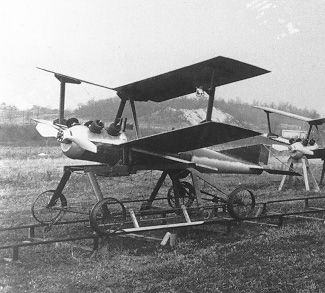
\includegraphics[width=0.5\textwidth]{kettering_bug.jpg}
    \caption{The Kettering Bug (1918).}
    \label{fig:ketteringbug}
\end{figure}

Throughout the 20th century, UAVs became more and more sophisticated, and were used more and more, but always for military purposes. In the more recent years, civilian UAVs have started to appear on the markets and their number quickly exceeded that of military UAVs. In February 2017, the FAA (Federal Aviation Administration) of the United States estimated that around 1.1 million units were in use in the US alone, and expected that number to rise to 3.55 million by 2021 \cite{consumerdronesbythenumbers}. These civilian drones are very different from military drones, in both their form and their function: civilian drones are usually smaller, and use rotors to take off vertically. They are used in a wide variety of applications.

\section{Motivation}
The ability to remote-control small and agile flying objects over large distances through the air, and to bring them to previously inaccessible locations, makes many new things possible. With the increasingly lower prices and better performances of civilian UAVs, people keep finding more and more uses for these high-tech gadgets. Some examples of these applications are: crop monitoring in agriculture \cite{agriculturaldrones}, delivery of mail or parcels, construction \cite{batiravecdesdrones}, cinematography, entertainment, or search and rescue operations. In all these applications, the more autonomous a drone is, the more efficient it will be at its task. One of the main challenges to achieve autonomy is for an UAV to be able to correctly identify its surroundings, and localize itself within them. In outdoor environments, GPS systems allow UAVs to know their position with great accuracy, but this is not possible in GPS-denied environments, like inside buildings. The main subject of this thesis will be fully autonomous navigation by a quadcopter in a GPS-denied environment.

\subsection{Ethical considerations}
The new possibilities brought by drones also pose ethical questions about security and privacy. Even though this technology can improve people's quality of life, it also has the potential to diminish it. If drones start to be widely used commercially, we could reach a point where the sound nuisances that they cause seriously impacts people who live in densely populated areas. Moreover, they can make us feel less at home, knowing that we could be observed from the sky at any moment. For this reason, it is important to adopt strict regulations regarding the use of drones in public spaces. Fortunately, many countries are already adopting legislation in this direction.


\section{Context}
This thesis is part of a project at the UCL that spans over several years and several masters theses. This project was launched by professor Julien Hendrickx in the 2012-2013 academic year, and has as long-term goal to develop a program that would enable low-cost UAVs to navigate autonomously in indoor environments. This means creating a map of their environment, localizing themselves in this map, and avoiding obstacles during exploration, using only on-board sensors. Another goal is to allow several drones to collaborate to speed up exploration. Five masters theses have already been written on this subject, each taking the work of the previous a little further.

\subsubsection{2012-2015: First three theses}
In each of the three academic years (2012-2013, 2013-2014, 2014-2015), a masters thesis on the subject of indoor navigation for autonomous low-cost drones was written. These masters theses formed the basis for subsequent work. They implemented visual SLAM methods to allow drones to build a two-dimensional map based on keypoints (first the keypoints were red pucks placed in advance, then visual landmarks that the drone detected from a textured scene), and to localize itself within this map. During this time, inter-drone communication was also established, and was used to allow a drone to communicate the location of a target to another drone.

\subsubsection{2015-2016: Recent work}
Last year, two groups of students simultaneously wrote theses within this project. Before doing so, they joined forces to re-implement all the existing code, but using ROS, a toolkit to develop software for robots that would make many things simpler, and allow more flexibility (see section \ref{sssec:ROS}).
The work of the first group of students allowed a drone to search and follow a mobile target, and call a second drone to replace it and continue this task when its battery was low.\\

The second group of students extended the SLAM algorithm to allow to use a 3D map to localize the drone. Unfortunately, they did not implement triangulation, so instead of projecting points into 3D space, they only used the drone's bottom-facing camera, and made the assumption that all points seen were located on the ground. The end result was a drone capable of using a 3D map to localize itself, but unable to build one from its observations.


\section{Objectives}
For this thesis, the goal is to continue the work of last year's second group to allow true 3-D SLAM: to build a 3D map based on observations by the monocular camera. To achieve this goal we will follow these intermediate objectives:
\begin{itemize}
\item Research the current state of the art for 3D keyframe-based monocular visual SLAM
\item Study how the drone can estimate its position by using a 3D map
\item Implement a way to triangulate points based on multiple observations
\item Implement a way to use new visual information to correct previous errors and build a consistent map
\item Provide improvements to the current code aiming for performance, speed, modularity, and readability
\end{itemize}


\section{Resources}
For the practical part of this project, we worked with a Parrot AR.Drone and various open-source software.

\begin{figure}[H]
  \centering
  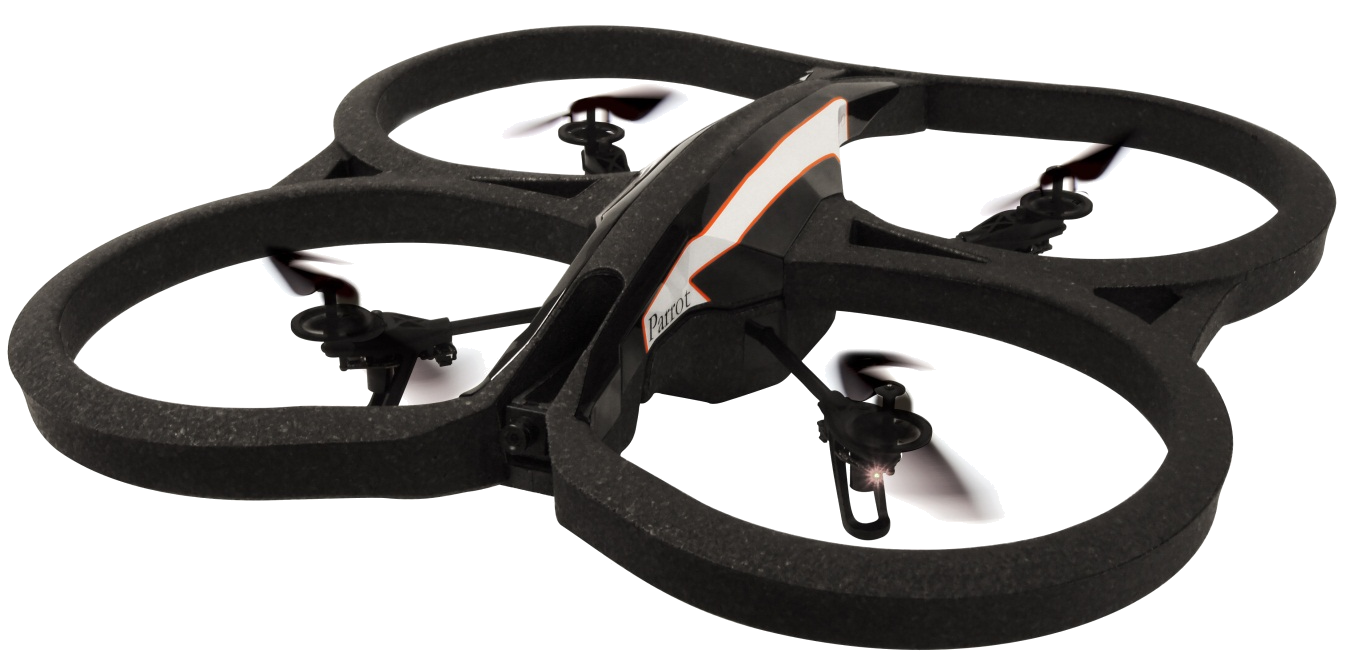
\includegraphics[width=0.5\textwidth]{ardrone.png}
    \caption{The Parrot AR.Drone}
    \label{fig:ardrone}
\end{figure}


\subsection{Hardware}
The Parrot AR.Drone 2.0 that we used was commercialized in 2012 and is an updated version of the original AR.Drone that was launched in 2010. This drone was marketed as a high tech toy, and is designed to be controlled from a smartphone application (connected to the drone via Wi-Fi). A few augmented reality games are available for the AR.Drone, in which it can visually recognize some predefined tags using its cameras, and interact with objects or other drones with a tag. To encourage the creation of more games for their drones, Parrot has released an open SDK that allows to effectively reprogram the drones. This early release of an open SDK has made it quite popular in the scientific community to perform research on autonomous flight. The drone consists of 4 rotors, each with their own electric motor and microcontroller, an internal computer with a 1GHz ARM Cortex A8 processor and 1GB DDR2 RAM at 200MHz, and various sensors.

\subsubsection{Sensors}
The AR.drone has the following sensors:
\begin{itemize}
  \item 3 axis accelerometer with $\pm$  \SI{50}{\milli\gram} accuracy
  \item 3 axis gyroscope with $\pm$ \SI{2000}{\degree\per\second} accuracy
  \item Pressure sensor with $\pm$ \SI{10}{\pascal} accuracy
  \item 3 axis magnetometer with $\pm$ \SI{6}{\degree} accuracy
  \item Ultrasound sensor (facing downwards)
  \item Front camera (HD 720p 30 fps)
  \item Bottom camera (QVGA, 60 fps)
\end{itemize}

The accelerometer and gyroscope form the IMU, or Inertial Measurement Unit. During normal (remote-controlled) operation, the IMU is used to estimate the speed of the drone, and stabilize it. The pressure sensor has a precision of \SI{10}{\pascal}, which is equivalent to about \SI{83}{\centi\metre} of air, so it is not precise enough to be a useful sensor indoors. Instead, the ultrasound sensor gives a very precise measurement of the altitude of the drone, but it only measures a distance in a single direction. The magnetometer is used along with the IMU to estimate the drone's orientations. The bottom camera is used to estimate the drone's speed, by using optical flow methods.

\subsubsection{Front Camera}
The front camera is not intended to be used as a sensor. During normal operation of the drone, its use is only for the user to be able to see through the drone, and make films or take pictures. In this work, however, we will use the front camera as the main sensor of our Simultaneous Localization and Mapping (SLAM) algorithm, to detect and map visual features. In indoor environments, the front camera is the drone's sensor that has the potential to capture the most information about its surroundings, as unlike the ultrasound sensor, it gives information in an entire area. Its field of view is also usually larger than the bottom camera's, because its scene is farther away. Because it is directed towards the front, it can see where the drone will go to, and so detect potential obstacles. Unfortunately, this information comes in the form of images, and deducing useable information from these images is not a trivial task, and requires computationally expensive algorithms. The main focus of this work will be to transform the images seen by this camera into useable information.

\subsubsection{Computational power}
The drone can communicate with an external computer through a Wi-Fi connection (the same that is used to connect it to a smartphone for a remote-controlled flight). For simplicity and to accelerate the development phase, we run our code on an external computer, communicating camera and other sensor readings from the drone to the computer, and commands from the computer to the drone. This is contradictory with the fact that the drone should be autonomous, but we could theoretically move the code on the drone for it to be executed on-board. Even though the computer we are using in the lab has a \SI{3.2}{\giga\hertz} quad-core processor, and is much faster than the embedded computer of the drone, it is realistic for our code to run in real time on an embedded computer, as today there exist cheap embedded computers that are much faster, than the ones included in the AR.Drone. Moreover, the most computationally expensive algorithms we run can be significantly sped up by using a graphics card, which we are not doing at the moment. There also exist graphics cards light enough to be embedded on a flying drone.

\subsection{Software}

\subsubsection{Closed-source internal code}\label{sec:closedsource}
The code that runs on the drone during normal execution is unfortunately closed-source. This code receives a velocity command from the user via a smartphone app, and drives the drone according to this input. When no input is given, the drone stays stationary, in "hover mode". To achieve this, it fuses sensor information from the IMU, the ultrasound, pressure sensor, magnetometer, as well as odometry from the optical flow of the bottom camera to estimate its displacement, and uses this fused pose estimate to stabilize itself.

\subsubsection{Parrot SDK}
The software development kit released by Parrot allows to send commands and receive information from the drone. It is possible to send the drone commands to take off, land, emergency stop, hover, or move at a certain speed in a certain direction, and it is possible to receive the drone's pose estimate. In both cases, however, the drone works as a black box: we can't directly control the command sent to the motors, and we don't have access at the control law used for the hover mode and for speed control. Similarly, we don't have access to the code estimating the drone's speed from optical flow, or to the data fusion that it does from all it's internal sensor readings.

\subsubsection{ROS}\label{sssec:ROS}
When programming the drone for the practical part of this project, we used the ROS (robot operating system) toolbox. All the previous work was already translated last year to use ROS. This toolbox provides useful abstraction to program robots: the program is decomposed into "nodes", each node running simultaneously in a separate thread. Each node implements part of the drone's task, and the nodes can communicate between each other by sending structured messages. The objective is to make the code general and modular, both at development level, by being able to make nodes that work with different kinds of robots, and reuse existing nodes created by other developers, and at runtime level, by being able to run only certain nodes at a time to test each part of the program separately. This also allows for collaboration between ROS's users. One existing ROS package is called "ardrone autonomy" \cite{ardroneautonomy}. This package was developed by the Autonomy Lab of Simon Fraser University and contains a node that handles communication with a physical AR.Drone. By using this node, we can completely disregard Parrot's specific SDK, and send all commands in ROS message format. This way, we hope to make it easy to reuse code in case future contributors to this project decide to change the hardware. ROS also provides a number of convenient tools for developing software to be used on robots, for example, it provides ways to record and replay data, and to easily set and change parameters, even during operation.

\subsubsection{OpenCV}
OpenCV is an open-source computer vision library. It provides functions and data structures to manipulate images, and implements many state-of-the-art computer vision algorithms. It can work with ROS messages. We will use this library for all of our computer vision implementation: keypoint detection, tracking, description, and matching.

\subsubsection{PCL}
PCL stands for Point Cloud Library and is an open-source library for 3D point cloud processing. The map created by the drone is a point cloud, and is saved as a PCL data structure. Currently, PCL is only used to store and visualize this map, but in the future, it can be used for higher-level functions like combining maps created by multiple robots, or reconstructing a dense representation of the map from a point cloud.

\subsubsection{Ceres Solver}
Ceres solver \cite{ceres-solver} is an open-source library for modeling and solving non-linear least squares problems. It was first created to solve bundle adjustment problems, but is now a general nonlinear optimization solver. It is developed and maintained by Google, where it is used for a variety of applications, for example to estimate the pose of the Google street cars and solve bundle adjustment problems in project Tango (Google's augmented reality project). It was released to the public as open-source software in 2012 \cite{introducingceres}. It will be used in this thesis to solve bundle adjustment problems (see section \ref{sec:bundleadjustment}).

\section{Constraints}
For the development part of this work, we were hindered by a few constraints:
\begin{itemize}
\item We have no way to measure the ground truth of the drone's position. It would be greatly useful to have an external sensor able to tell the position of the drone precisely to compare it to the one the drone estimates.
\item The lights in the lab where we carried out our tests are neon lights, which flicker at a high frequency. The frequency of this flickering leads to an aliasing effect on the camera's image.
\item Parrot's internal software is closed-source, and we don't have access to some sensors (like the ultrasound) when the drone isn't flying.
\end{itemize}

\section{Outline}
First, the state of the art of miniature UAVs, computer vision, and simultaneous localization and mapping will be explored in chapter 2. Chapters 3 through 5 will present the main subject of this work: computer vision (Chapter 3), localization (Chapter 4), mapping (Chapter 5). Each of these sections explains the theory behind that part of the task, and ends with a small summary and a flowchart outlining the organization of the code for that part. A general outline showing how the different parts of the program work together can be found in appendix \ref{app:flowchart}. The main results will then be presented in chapter 6. Finally, chapter 7 will expose the main conclusions of this thesis, and describe the main challenges for further work on this project.
